\documentclass[a4paper,11pt]{book}
\usepackage{listings}
\usepackage{xspace}
\usepackage{url}
\usepackage[utf8]{inputenc}
\usepackage[spanish]{babel}

%\usepackage[style=list, number=none]{glossary} %
%\usepackage{titlesec}
%\usepackage{pailatino}

\decimalpoint
\usepackage{dcolumn}
\newcolumntype{.}{D{.}{\esperiod}{-1}}
\makeatletter
\addto\shorthandsspanish{\let\esperiod\es@period@code}
\makeatother


%\usepackage[chapter]{algorithm}
\RequirePackage{verbatim}
%\RequirePackage[Glenn]{fncychap}
\usepackage{fancyhdr}
\usepackage{graphics, graphicx, float}
\usepackage{afterpage}

\usepackage{longtable}

\usepackage[pdfborder={000}]{hyperref} %referencia

% ********************************************************************
% Re-usable information
% ********************************************************************
\newcommand{\myTitle}{3DCurator\xspace}
\newcommand{\mySubtitle}{Un visor 3D de TACs de esculturas\xspace}
\newcommand{\myDegree}{Grado en Ingeniería Informática\xspace}
\newcommand{\myName}{Francisco Javier Bolívar Lupiáñez\xspace}
\newcommand{\myProf}{Francisco Javier Melero Rus\xspace}
\newcommand{\myFaculty}{Escuela Técnica Superior de Ingenierías Informática y de Telecomunicación\xspace}
\newcommand{\myFacultyShort}{E.T.S. de Ingenierías Informática y de Telecomunicación\xspace}
\newcommand{\myDepartment}{Departamento de Lenguajes y Sistemas Informáticos\xspace}
\newcommand{\myUni}{\protect{Universidad de Granada}\xspace}
\newcommand{\myLocation}{Granada\xspace}
\newcommand{\myTime}{\today\xspace}
\newcommand{\myVersion}{Version 0.1\xspace}


\hypersetup{
pdfauthor = {\myName (fblupi@correo.ugr.es)},
pdftitle = {\myTitle},
pdfsubject = {},
pdfkeywords = {palabra_clave1, palabra_clave2, palabra_clave3, ...},
pdfcreator = {LaTeX con el paquete ....},
pdfproducer = {pdflatex}
}

%\hyphenation{}


%\usepackage{doxygen/doxygen}
%\usepackage{pdfpages}
\usepackage{url}
\usepackage{colortbl,longtable}
\usepackage[stable]{footmisc}
%\usepackage{index}

%\makeindex
%\usepackage[style=long, cols=2,border=plain,toc=true,number=none]{glossary}
% \makeglossary

% Definición de comandos que me son tiles:
%\renewcommand{\indexname}{Índice alfabético}
%\renewcommand{\glossaryname}{Glosario}

\pagestyle{fancy}
\fancyhf{}
\fancyhead[LO]{\leftmark}
\fancyhead[RE]{\rightmark}
\fancyhead[RO,LE]{\textbf{\thepage}}
\renewcommand{\chaptermark}[1]{\markboth{\textbf{#1}}{}}
\renewcommand{\sectionmark}[1]{\markright{\textbf{\thesection. #1}}}

\setlength{\headheight}{1.5\headheight}

\newcommand{\HRule}{\rule{\linewidth}{0.5mm}}
%Definimos los tipos teorema, ejemplo y definición podremos usar estos tipos
%simplemente poniendo \begin{teorema} \end{teorema} ...
\newtheorem{teorema}{Teorema}[chapter]
\newtheorem{ejemplo}{Ejemplo}[chapter]
\newtheorem{definicion}{Definición}[chapter]

\definecolor{gray97}{gray}{.97}
\definecolor{gray75}{gray}{.75}
\definecolor{gray45}{gray}{.45}
\definecolor{gray30}{gray}{.94}

\lstset{ frame=Ltb,
     framerule=0.5pt,
     aboveskip=0.5cm,
     framextopmargin=3pt,
     framexbottommargin=3pt,
     framexleftmargin=0.1cm,
     framesep=0pt,
     rulesep=.4pt,
     backgroundcolor=\color{gray97},
     rulesepcolor=\color{black},
     %
     stringstyle=\ttfamily,
     showstringspaces = false,
     basicstyle=\scriptsize\ttfamily,
     commentstyle=\color{gray45},
     keywordstyle=\bfseries,
     %
     numbers=left,
     numbersep=6pt,
     numberstyle=\tiny,
     numberfirstline = false,
     breaklines=true,
   }
 
% minimizar fragmentado de listados
\lstnewenvironment{listing}[1][]
   {\lstset{#1}\pagebreak[0]}{\pagebreak[0]}

\lstdefinestyle{CodigoC}
   {
	basicstyle=\scriptsize,
	frame=single,
	language=C,
	numbers=left
   }
\lstdefinestyle{CodigoC++}
   {
	basicstyle=\small,
	frame=single,
	backgroundcolor=\color{gray30},
	language=C++,
	numbers=left
   }

 
\lstdefinestyle{Consola}
   {basicstyle=\scriptsize\bf\ttfamily,
    backgroundcolor=\color{gray30},
    frame=single,
    numbers=none
   }


\newcommand{\bigrule}{\titlerule[0.5mm]}


%Para conseguir que en las páginas en blanco no ponga cabecerass
\makeatletter
\def\clearpage{%
  \ifvmode
    \ifnum \@dbltopnum =\m@ne
      \ifdim \pagetotal <\topskip
        \hbox{}
      \fi
    \fi
  \fi
  \newpage
  \thispagestyle{empty}
  \write\m@ne{}
  \vbox{}
  \penalty -\@Mi
}
\makeatother

\usepackage{pdfpages}
\begin{document}
\begin{titlepage}
 
\newlength{\centeroffset}
\setlength{\centeroffset}{-0.5\oddsidemargin}
\addtolength{\centeroffset}{0.5\evensidemargin}
\thispagestyle{empty}

\noindent\hspace*{\centeroffset}
\begin{minipage}{\textwidth}
\centering

\includegraphics[width=0.9\textwidth]{imagenes/logo_ugr.jpg}\\[1.4cm]
\textsc{ \Large TRABAJO FIN DE GRADO\\[0.2cm]}
\textsc{ INGENIERÍA EN INFORMÁTICA}\\[1cm]
{\Huge\bfseries \myTitle \\}
\noindent\rule[-1ex]{\textwidth}{3pt}\\[3.5ex]
{\large\bfseries \mySubtitle}
\end{minipage}

\vspace{2.5cm}

\noindent\hspace*{\centeroffset}
\begin{minipage}{\textwidth}
\centering
\textbf{Autor}\\ {\myName}\\[2.5ex]
\textbf{Director}\\ {\myProf}\\[2cm]

\includegraphics[width=0.3\textwidth]{imagenes/etsiit_logo.png}\\[0.1cm]
\textsc{\myFaculty}\\
\textsc{---}\\
\myLocation, \myTime
\end{minipage}

\end{titlepage}



\chapter*{}

\begin{titlepage}
 
 
\setlength{\centeroffset}{-0.5\oddsidemargin}
\addtolength{\centeroffset}{0.5\evensidemargin}
\thispagestyle{empty}

\noindent\hspace*{\centeroffset}
\begin{minipage}{\textwidth}
\centering
\vspace{3.3cm}
%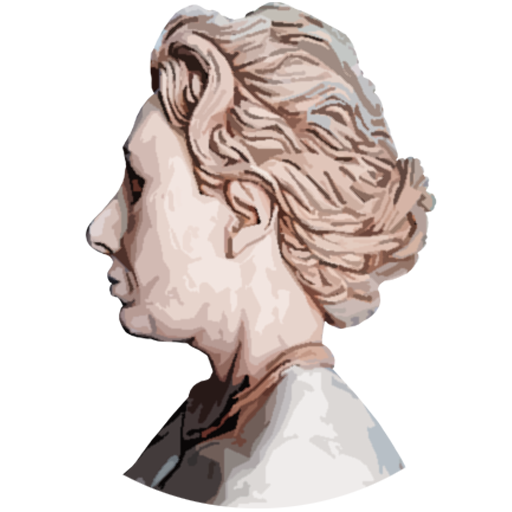
\includegraphics{imagenes/logo.png} 
%\vspace{0.5cm}

{\Huge\bfseries \myTitle \\}
\noindent\rule[-1ex]{\textwidth}{3pt}\\[3.5ex]
{\large\bfseries \mySubtitle \\[4cm]}
\end{minipage}

\vspace{2.5cm}

\noindent\hspace*{\centeroffset}
\begin{minipage}{\textwidth}
\centering
\textbf{Autor}\\ {\myName}\\[2.5ex]
\textbf{Director}\\ {\myProf}\\[2cm]
\end{minipage}

\vspace{\stretch{2}}

\end{titlepage}




\cleardoublepage
\thispagestyle{empty}

\begin{center}
{\large\bfseries \myTitle: \mySubtitle}\\
\end{center}

\begin{center}
\myName \\
\end{center}

\vspace{0.7cm}
\noindent{\textbf{Palabras clave}: palabra\_clave1, palabra\_clave2, palabra\_clave3, ......}\\

\vspace{0.7cm}
\noindent{\textbf{Resumen}}\\

Poner aquí el resumen.

\chapter*{}
\thispagestyle{empty}

\noindent\rule[-1ex]{\textwidth}{2pt}\\[4.5ex]

Yo, \textbf{\myName}, alumno de la titulación \myDegree de la \textbf{\myFaculty}, con DNI 75926571Y, autorizo la ubicación de la siguiente copia de mi Trabajo Fin de Grado en la biblioteca del centro para que pueda ser consultada por las personas que lo deseen.

\vspace{6cm}

\noindent Fdo: \myName

\vspace{2cm}

\begin{flushright}
\myLocation a \myTime.
\end{flushright}


\chapter*{}
\thispagestyle{empty}

\noindent\rule[-1ex]{\textwidth}{2pt}\\[4.5ex]

D. \textbf{\myProf}, Profesor del Área de XXXX del \myDepartment de la \myUni.

\vspace{0.5cm}

\textbf{Informa:}

\vspace{0.5cm}

Que el presente trabajo, titulado \textit{\textbf{\myTitle, \mySubtitle}}, ha sido realizado bajo su supervisión por \textbf{\myName}, y autorizamos la defensa de dicho trabajo ante el tribunal que corresponda.

\vspace{0.5cm}

Y para que conste, expiden y firman el presente informe en \myLocation a \myTime.

\vspace{1cm}

\textbf{El director:}

\vspace{5cm}

\noindent \textbf{\myProf}

\chapter*{Agradecimientos}
\thispagestyle{empty}

\vspace{1cm}

Poner aquí agradecimientos...


\frontmatter
\tableofcontents
\listoffigures
\listoftables
%
\mainmatter
\setlength{\parskip}{5pt}

\chapter{Introducción}
El objetivo de este proyecto es construir un software con el que poder visualizar e interactuar con los datos DICOM obtenidos al someter a una escultura a una Tomografía Axial Computerizada (TAC). 

Para ello se hará uso de VTK, que proporciona una serie de librerías en C++ para facilitar operaciones sobre datos DICOM, y de Qt, para la Interfaz Gráfica de Usuario (GUI).

Antes de empezar con el proyecto en sí, se definirán conceptos como DICOM o TAC que se usarán a lo largo de éste y conviene saber lo que son, así como las distintas herramientas que se utilizarán.

\section{Obtención de datos DICOM mediante un TAC}
DICOM (\textit{Digital Imaging and Comunication in Medicine}) es el estándar internacional para manejar, visualizar, almacenar, imprimir y transmitir imágenes de pruebas médicas (ISO12052) \cite{about_dicom}. 

Al contrario de lo que se puede pensar en un principio, DICOM es más que un formato de imagen, es un protocolo que abarca la transferencia, el almacenamiento y la visualización \cite{dicom_intro_and_guide}.

Pese a que su uso está mayoritariamente extendido en el campo en el que nació (la medicina), se puede usar en otros, como el de la restauración de bienes culturales, como es el caso de este proyecto.

En un archivo DICOM hay almacenado, además de metadatos, una imagen \cite{dicom_classes_vtk} (Figura \ref{fig:prostate_dicom}).

\begin{figure}[H]
	\centering
	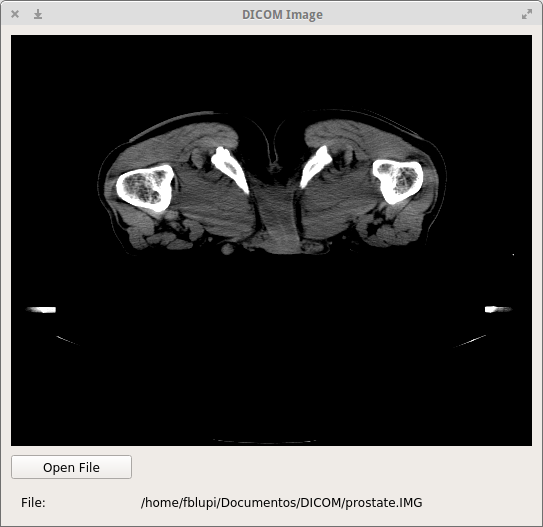
\includegraphics[width=10cm]{imagenes/prostate_dicom}
	\caption{Imagen DICOM de una próstata visualizada con un programa diseñado para visualizar archivos DICOM.}
	\label{fig:prostate_dicom}
\end{figure}

\begin{figure}[H]
	\centering
	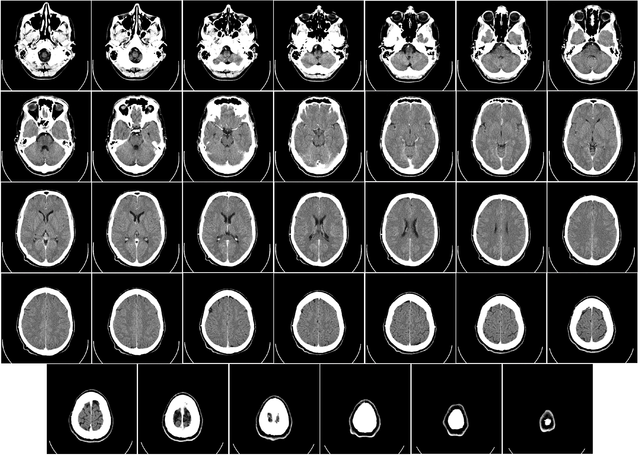
\includegraphics[width=10cm]{imagenes/brain_dicom_serie}
	\caption{Serie de imágenes DICOM extraídas de un TAC realizada a un cerebro.}
	\label{fig:brain_dicom_serie}
\end{figure}

Cuando se realiza un escáner TAC (Tomografía Axial Computerizada) se obtiene una serie de imágenes (Figura \ref{fig:brain_dicom_serie}) de rebanadas del objeto al que se le realiza el escáner. Éstas imágenes se encapsulan en archivos DICOM, y con todas ellas se puede llegar a construir un modelo volumétrico.

El cómo se obtienen las imágenes con un TAC no es objeto de estudio de este proyecto, por lo que no se entrará en mucho detalle. En muy resumidas cuentas, el aparato emite un haz de rayos X desde distintos ángulos al objeto y unos sensores recogen la radiación que absorbe en cada una de estas emisiones. Obteniendo el resultado final del promedio de todas las mediciones que realizan los sensores \cite{tac}. 
\chapter{Especificación de requisitos}

Este capítulo es una Especificación de Requisitos Software para el software que se va a realizar siguiendo las directrices dadas por el estándar IEEE830 \cite{iee830}.

\section{Introducción}

	\subsection{Propósito}
	
	Este capítulo de especificación de requisitos tiene como objetivo definir las especificaciones funcionales y no funcionales para el desarrollo de un software que permitirá visualizar e interactuar con los datos DICOM obtenidos al someter a una escultura a una TC. Éste software será utilizado principalmente por restauradores.
	
	\subsection{Ámbito del sistema}
	
	En la actualidad los datos DICOM obtenidos tras una TC se utilizan, principalmente, en el campo donde surgieron, la medicina. No obstante, esto no significa que solo se pueda aplicar ahí. Con este software, llamado \myTitle, se tratará de trasladar esta técnica al campo de la restauración de bienes culturales y poder visualizar e interactuar con los datos DICOM obtenidos con esculturas.
	
	\subsection{Definiciones, acrónimos y abreviaturas}
	
	\begin{itemize}
		\item \textbf{ERS}: Especificación de Requisitos Software.
		\item \textbf{GUI} (\textit{Graphic User Interface}): Interfaz gráfica de usuario.
		\item \textbf{DICOM} (\textit{Digital Imaging and Comunication in Medicine}): Datos de donde se obtienen las imágenes.
		\item \textbf{TAC o TC} (Tomografía Axial Computerizada): Escáner en el que se obtienen los datos DICOM.
		\item \textbf{GPU} (\textit{Graphic Precessor Unit}): Tarjeta gráfica.
		\item \textbf{VTK} (\textit{The Visualization ToolKit}): Librería gráfica que se utilizará.
		\item \textbf{CMake} (\textit{Cross platform Make}): Herramienta para generar código compilable en distintas plataformas.
		\item \textbf{Qt}: Librería que se utilizará para realizar la GUI.
		\item \textbf{Volumen}: Conjunto de datos en los que para cada posición XYZ se tiene un valor determinado.
		\item \textbf{Corte}: Vista de la figura a través de un plano. Por ejemplo, al cortar con una sierra un tronco por la mitad, se puede ver cómo es por dentro en esa posición por donde se ha cortado.
		\item \textbf{Función de transferencia}: Función utilizada para visualizar los datos deseados de un volumen.
		\item \textbf{\textit{Direct Volume Rendering}}: Visualización directa de volúmenes en la que cada valor del volumen se mapea con un determinado color y opacidad dado por una función de transferencia.
		\item \textbf{\textit{Ray-Casting}}: Técnica de \textit{Direct Volume Rendering} utilizada para la visualización de volúmenes.
		\item \textbf{\textit{Widget}}: Elemento de la GUI.
	\end{itemize}
	
	\subsection{Visión general del documento}
	
	Este capítulo consta de tres secciones:
	\begin{itemize}
		\item En la primera sección se realiza una introducción a éste y se proporciona una visión general de la ERS.
		\item En la segunda sección se realiza una descripción general a alto nivel del software, describiendo los factores que afectan al producto y a sus requisitos y con el objetivo de conocer las principales funcionalidades de éste.
		\item En la tercera sección se definen detalladamente los requisitos que deberá satisfacer el software.
	\end{itemize}

\section{Descripción general}

\subsection{Perspectiva del producto}

	El software \myTitle tiene como objetivo interactuar con datos DICOM, pero no es el encargado de generarlos. Para generarlos se deberá utilizar algún escáner de TC.
	
	Una vez obtenidos, no se necesitará ningún otro software adicional.
	
	\subsection{Funciones del producto}
	
	Las principales funcionalidades de este sistema serán:
	\begin{itemize}
		\item Cargar datos DICOM.
		\item Generar un volumen a partir de los datos cargados.
		\item Visualizar en 3D el volumen.
		\item Modificar la función de transferencia y cambiar colores asignados a cada material.
		\item Generar nuevos cortes.
		\item Visualizar los cortes generados.
		\item Guardar imagen de lo que se visualiza en la pantalla.
	\end{itemize}
	
	\subsection{Características de los usuarios}
	
	Solo existe un tipo de usuario, que es la persona que desee interactuar con los datos DICOM de una escultura. Esta persona no tiene por qué tener habilidad con un equipo informático, por lo que \myTitle deberá tener una GUI intuitiva y fácil de utilizar.
	
	\subsection{Restricciones}
	
	Se llevará a cabo un desarrollo evolutivo basado en un prototipo funcional en el que no están definidos todos los requisitos desde un principio y se irán añadiendo conforme se vayan completando y ocurriendo nuevos.
	
	El software será libre, por lo que el código estará accesible en un repositorio de GitHub.
	
	Se programará en C++ usando las librerías VTK para la visualización de gráficos y Qt para la GUI.
	
	Aprovechando que se debe usar CMake para compilar las librerías mencionadas, se utilizará también para generar el proyecto, pues se puede generar código compilable en distintas plataformas.
	
	\subsection{Suposiciones y dependencias}
	
	El software se utilizará para poder visualizar esculturas de madera por lo que se tendrán en cuenta los materiales con los que están hechas la mayoría de estas. Si se introducen los datos DICOM de cualquier otra cosa con materiales distintos a los utilizados en las esculturas no se visualizará correctamente.

\section{Requisitos específicos}

	\subsection{Interfaces}
	
	La GUI se construirá con Qt y contendrá los siguientes elementos (Figura \ref{fig:basic_gui}):
	\begin{itemize}
		\item \textbf{Barra de menú}: Típica barra de menús (archivo, editar, herramientas...).
		\item \textbf{Barras de herramientas}: Acceso rápido con los botones de las operaciones más utilizadas sobre cada \textit{widget} de visualización.
		\item \textbf{\textit{Widget} de visualización del volumen en 3D}: Con el que se podrá interactuar para girar, hacer zoom y ver la figura desde distintas posiciones.
		\item \textbf{\textit{Widget} de visualización de cortes}: En el que se mostrará el corte que se genera con un plano determinado.
		\item \textbf{Menú de operaciones}: Menú organizado en pestañas donde se podrán realizar distintas operaciones como cambiar la función de transferencia y definir el plano para realizar un corte.
	\end{itemize}
	
	\begin{figure}[H]
		\centering
		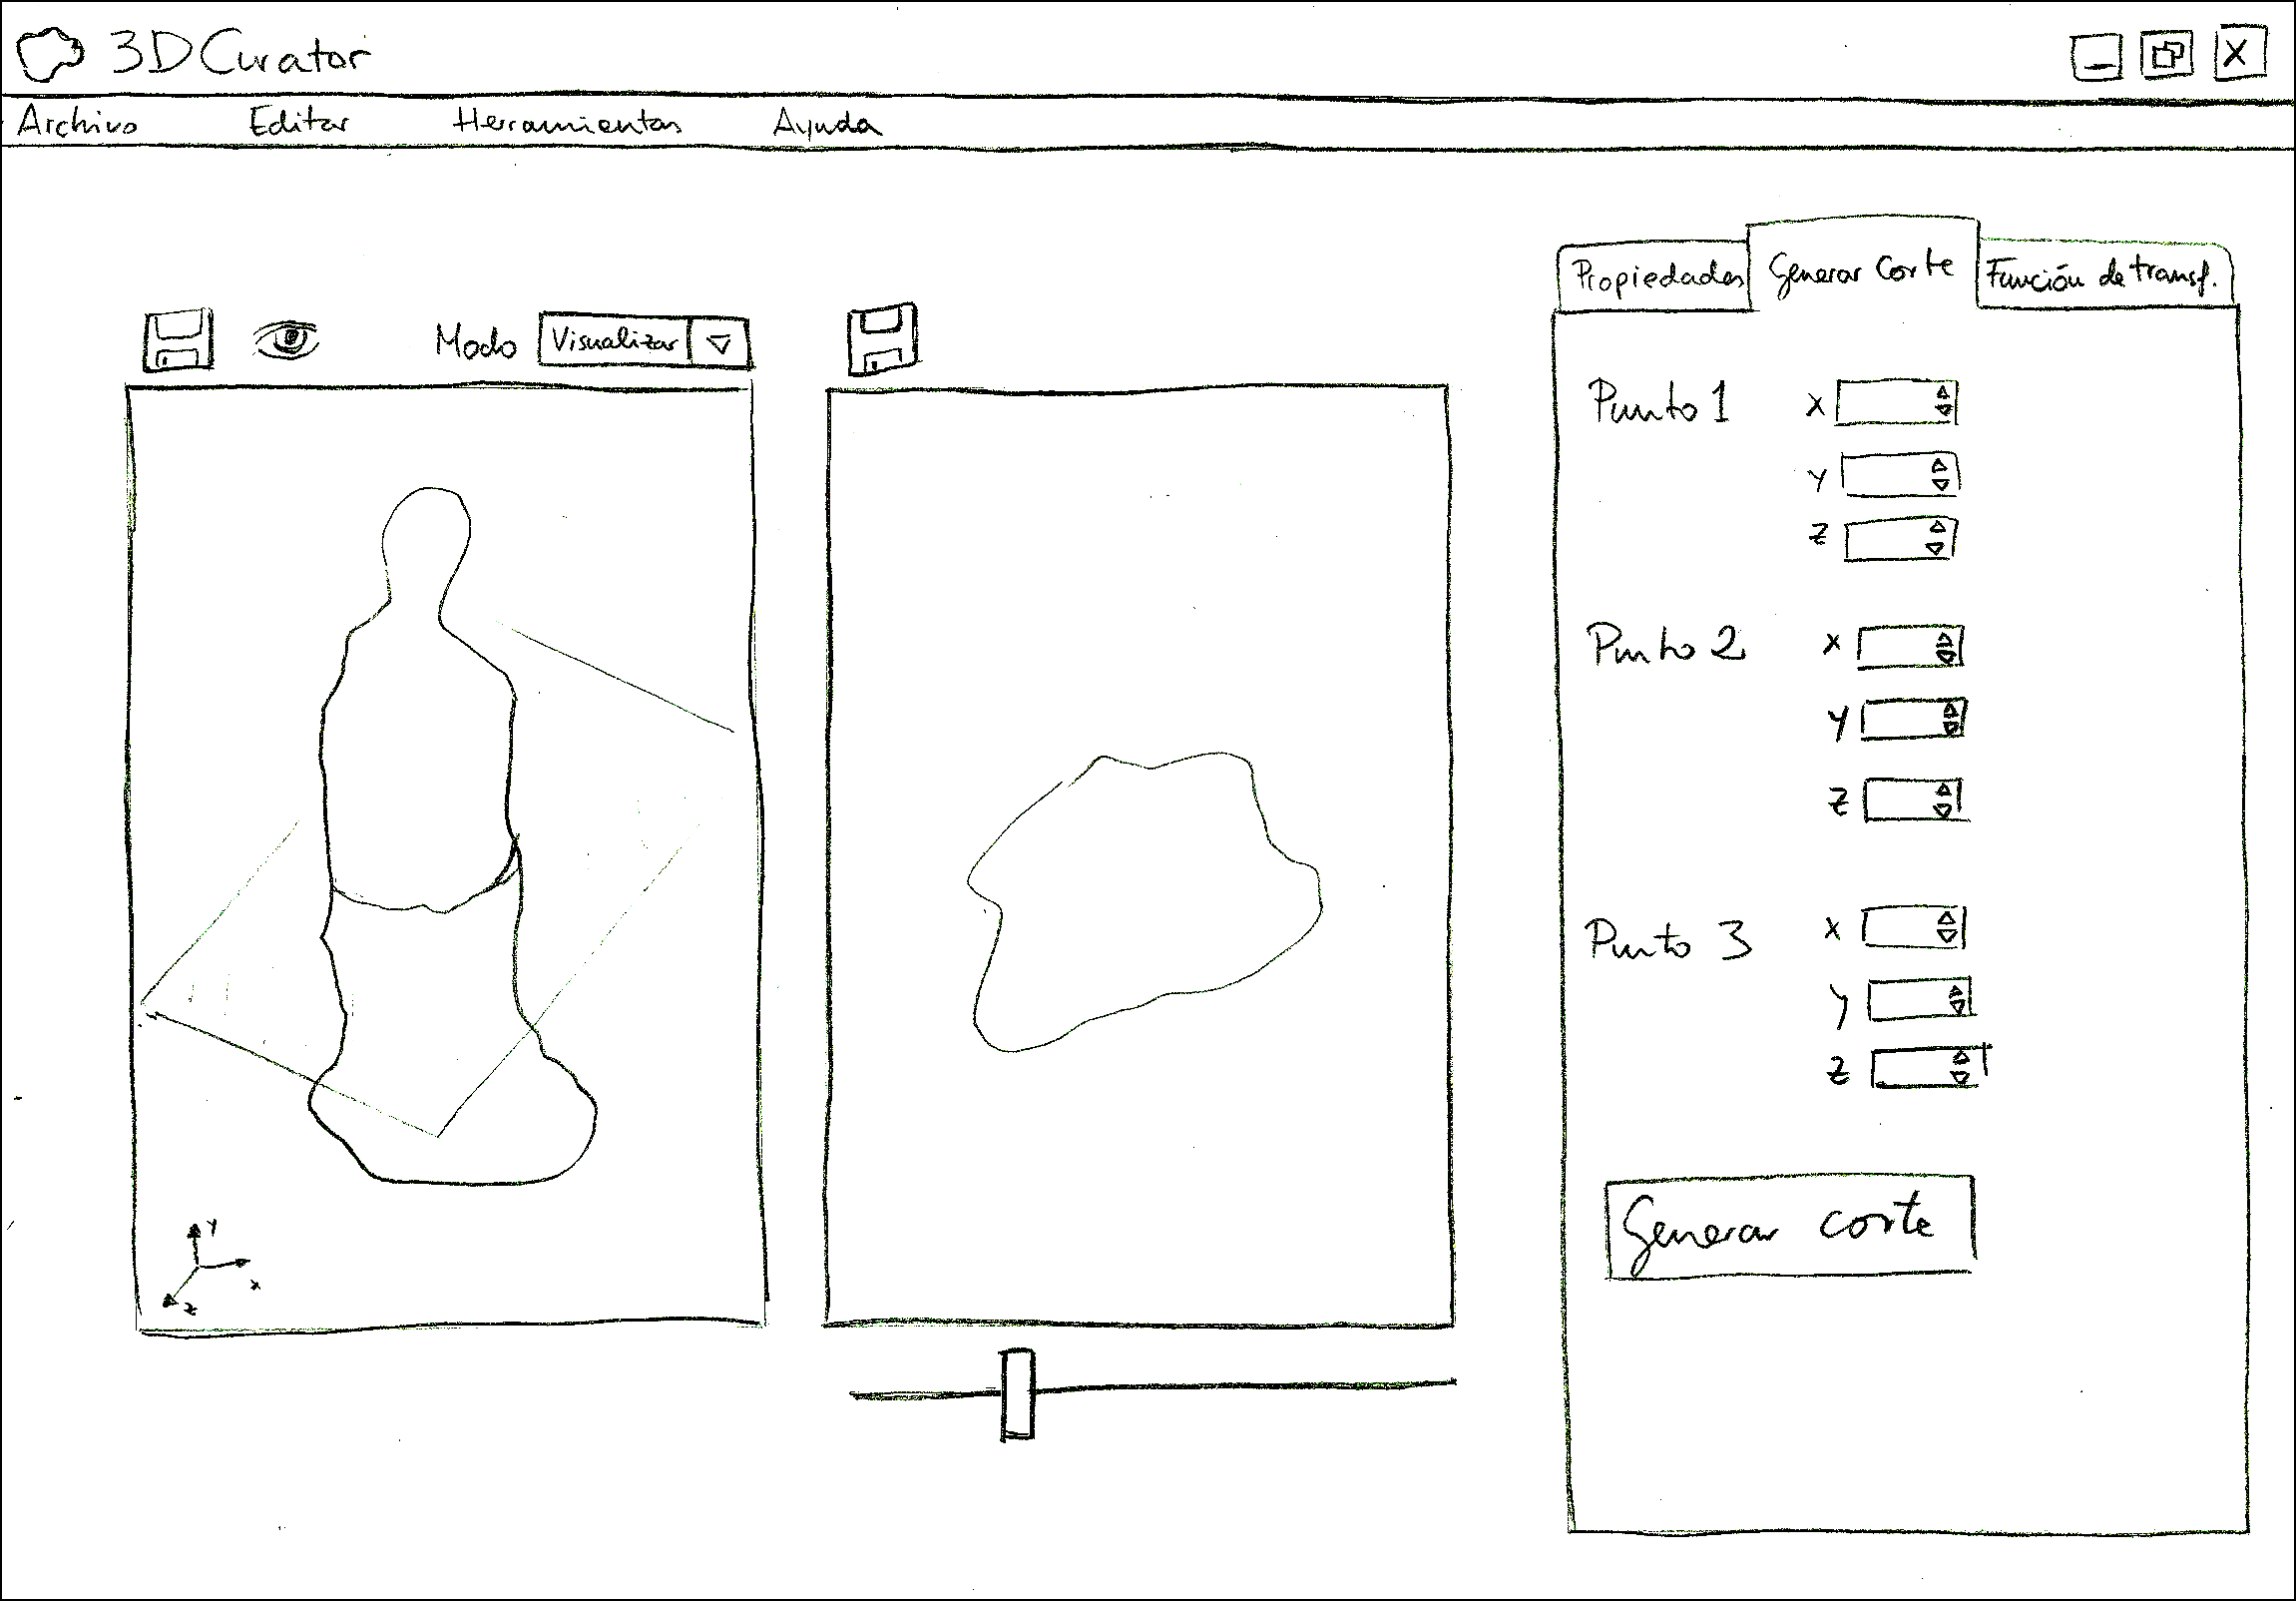
\includegraphics[width=12.5cm]{imagenes/basic_gui}
		\caption{Boceto a mano alzada de la posible distribución de los elementos en la GUI}
		\label{fig:basic_gui}
	\end{figure}
	
	\subsection{Funciones}
	
	El sistema tendrá que realizar distintas funciones que se comentaron anteriormente pero se profundizará en esta sección. Se han estructurado estas funciones por su objetivo separando cuatro subsecciones distintas: Lectura de datos, generación de cortes, visualización y configuración.
	
		\subsubsection{Lectura de datos}
		\begin{itemize}
			\item \textbf{Seleccionar carpeta}: Cuando el usuario quiera cargar datos DICOM, le aparecerá una ventana donde se podrá escoger alguna carpeta de su sistema de forma que solo muestre las carpetas y no los archivos.
			\item \textbf{Verificar que la carpeta contiene datos DICOM}: Se tendrá que verificar que el usuario ha seleccionado una carpeta con datos DICOM y se le avisará si no lo ha hecho.
			\item \textbf{Cargar datos DICOM}: Cuando se haya seleccionado una carpeta correcta, se cargarán los datos y automáticamente los visualizará en 3D con la configuración por defecto.
		\end{itemize}
	
		\subsubsection{Generación de cortes}
		\begin{itemize}
			\item \textbf{Definir plano}: El usuario podrá definir un plano por donde realizar un corte a la figura. Para ello tendrá que introducir tres puntos. Por defecto, se introducirá un plano en el eje XZ a una altura de Y = 0, siendo la dirección de los ejes XYZ la que utiliza VTK (Figura \ref{fig:vtk_axes}). El plano se podrá visualizar en el \textit{widget} de visualización 3D para ver gráficamente por dónde pasará.
			\begin{figure}[H]
				\centering
				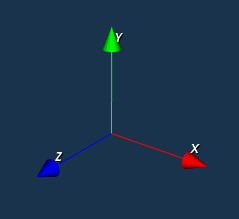
\includegraphics[width=8cm]{imagenes/vtk_axes}
				\caption{Dirección de los ejes XYZ}
				\label{fig:vtk_axes}
			\end{figure}
			\item \textbf{Modificar plano}: El usuario podrá modificar el plano o introduciendo nuevos puntos, o interactuando con la vista previa de éste en el \textit{widget} de visualización 3D. Las operaciones que podrá realizar en este serán:
			\begin{itemize}
				\item Rotar en cualquiera de los ejes.
				\item Trasladar en dirección de la normal.
			\end{itemize}
			\item \textbf{Generar corte}: Una vez se haya creado el plano deseado, se podrá mostrar el corte en el \textit{widget} de visualización de cortes.
		\end{itemize}
	
		\subsubsection{Visualización}
		\begin{itemize}
			\item \textbf{Visualizar en 3D}: Cuando el usuario haya seleccionado una carpeta con datos DICOM, se mostrará en 3D en el \textit{widget} izquierdo pudiendo rotar y hacer zoom interactuando con el ratón. Para visualizar el volumen se utilizarán técnicas de \textit{Direct Volume Rendering} que proporcionan VTK como puede ser el \textit{Ray-Casting}.
			\item \textbf{Visualizar corte}: Cuando el usuario haya cargado los datos DICOM y haya establecido un plano de corte, se podrá generar un corte a la figura por éste. Este corte se visualizará en el \textit{widget} derecho.
			\item \textbf{Guardar imagen}: El usuario en todo momento podrá guardar una imagen (en formatos comunes JPG o PNG) de lo que está viendo en cada uno de los \textit{widgets} seleccionando en una ventana que aparecerá cuando se elija la opción la dirección donde se guardará y el nombre del archivo. 
		\end{itemize}
	
		\subsubsection{Configuración}
		\begin{itemize}
			\item \textbf{Cambiar color de fondo}: El usuario podrá cambiar el color de fondo del \textit{widget} donde se mostrará la figura en 3D. Para ello podrá:
			\begin{itemize}
				\item Elegir entre colores predeterminados.
				\item Introducir un color mediante valores RGB.
				\item Introducir un color mediante su código de color hexadecimal.
			\end{itemize}
			\item \textbf{Cambiar función de transferencia}: El usuario podrá cambiar la función de transferencia utilizada para poder ver los distintos materiales con una paleta de color distinta a la que se da por defecto.
		\end{itemize}
	
	\subsection{Requisitos de rendimiento}
	
	Al ser una aplicación de escritorio donde no se almacenarán datos sino que se mostrarán, los requisitos de rendimiento no se centrarán en la concurrencia de acceso ni en el almacenamiento, como lo podrían estar en una aplicación web.
	
	Sin embargo, hay que tener en cuenta otros factores, como pueden ser el uso eficiente de memoria y no tener cargadas todas las figuras que se han estado visualizando, desechando la anterior cuando se carga una nueva.
	
	El rendimiento gráfico también es importante, por eso y para obtener imágenes de mayor calidad, se utilizarán técnicas de \textit{Direct Volume Rendering} como el \textit{Ray-Casting}. Estas técnicas necesitan una gran cantidad de procesamiento, pero la velocidad de procesamiento de las GPUs actuales no deberían resultar un problema.
	
	\subsection{Restricciones de diseño}
	
	Al utilizar la librería VTK se seguirá su estructura a la hora de construir el software, y se tendrán restricciones en cuanto a funcionalidad que se pueda construir con ésta. No obstante es una librería muy completa y no se debería encontrar ninguna restricción viendo otros programas de visualización de datos médicos que se han construido usando esta librería.
	
	\subsection{Atributos del software}
	
	Al usar CMake, se podrá crear un software multiplataforma que funcione en cualquier sistema operativo.
	
	El software generado deberá ser fiable, porque aunque no trabaje con datos sensibles cuya pérdida pueda ser grave, siempre resulta molesto utilizar un software con fallos que interrumpan durante su uso.
	
	También se debe tener en cuenta que el software sea mantenible pues, al ser libre, otros desarrolladores pueden colaborar en su desarrollo y debe estar bien documentado para que esto sea una tarea fácil.
%
%\input{capitulos/03_Planificacion}
%
%\input{capitulos/04_Analisis}
%
%\input{capitulos/05_Diseno}
%
%\input{capitulos/06_Implementacion}
%
%\input{capitulos/07_Pruebas}
%
%\input{capitulos/08_Conclusiones}
%
%%\chapter{Conclusiones y Trabajos Futuros}
%
%
%%\nocite{*}
\bibliography{bibliografia/bibliografia}
\addcontentsline{toc}{chapter}{Bibliografía}
\bibliographystyle{plain}
%
%\appendix
%\chapter{Manual de usuario}

\section{Requisitos}

\begin{itemize}
	\item Microsoft Windows 7 o superior
	\item Drivers gráficos compatibles con OpenGL 4
	\item 2GB RAM
\end{itemize}

\section{Instalación}

Instalar usando \texttt{3DCurator.msi} siguiendo los siguientes pasos:

\begin{figure}[H]
	\centering
	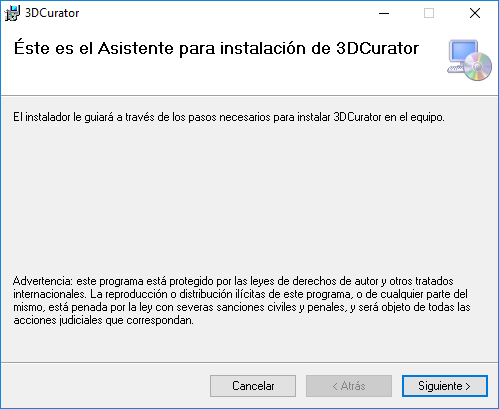
\includegraphics[width=9cm]{imagenes/instalacion_1}
	\caption{Hacer click en Siguiente}
	\label{fig:instalacion_1}
\end{figure}

\begin{figure}[H]
	\centering
	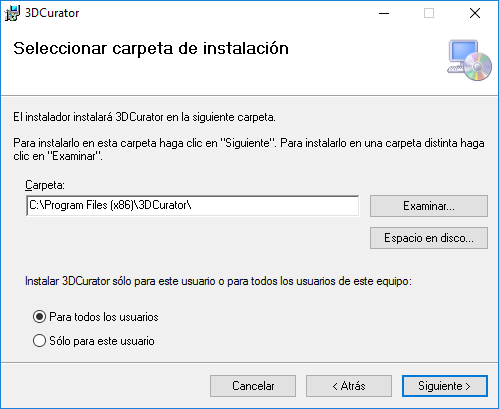
\includegraphics[width=9cm]{imagenes/instalacion_2}
	\caption{Hacer click en Siguiente o cambiar cualquiera de las opciones}
	\label{fig:instalacion_2}
\end{figure}

\begin{figure}[H]
	\centering
	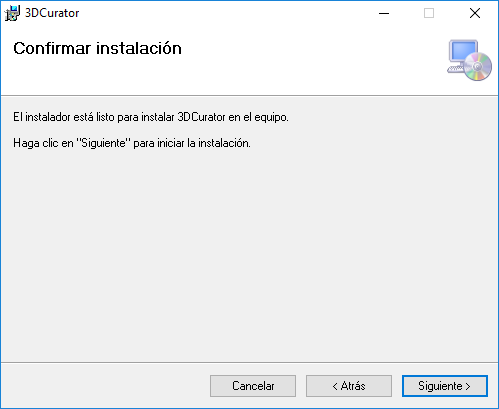
\includegraphics[width=9cm]{imagenes/instalacion_3}
	\caption{Hacer click en Siguiente,  dar permisos de administrador y comenzará a instalarse}
	\label{fig:instalacion_3}
\end{figure}

\begin{figure}[H]
	\centering
	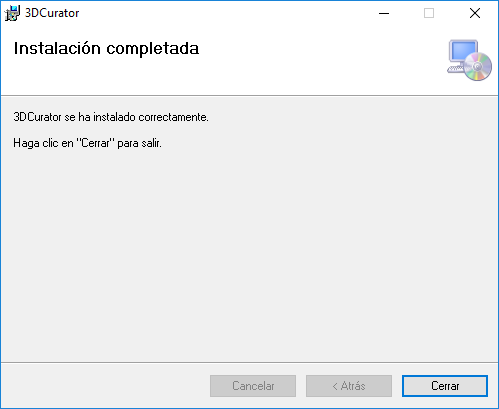
\includegraphics[width=9cm]{imagenes/instalacion_4}
	\caption{Hacer click en Cerrar. Al instalar se habrá creado un acceso directo en el escritorio y en el menú de inicio}
	\label{fig:instalacion_4}
\end{figure}

\section{Capturas de pantalla}

\begin{figure}[H]
	\centering
	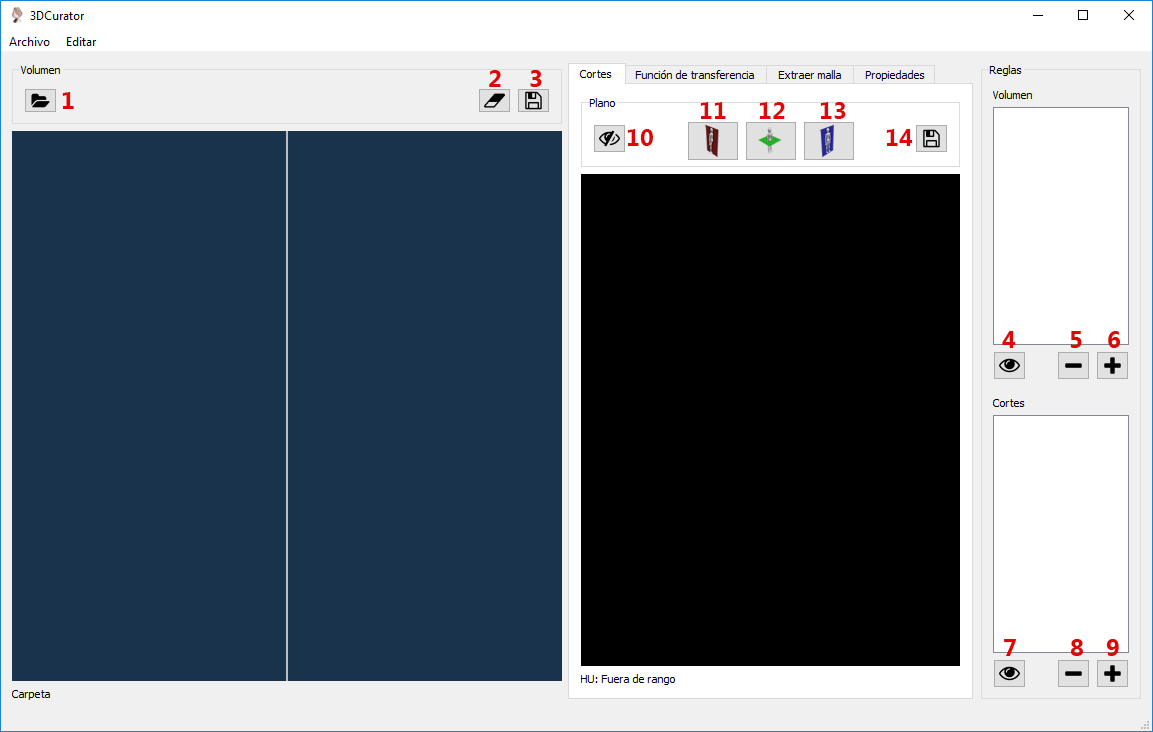
\includegraphics[width=12.5cm]{imagenes/gui_1}
	\caption{Captura de la GUI (Pestaña \textit{Cortes})}
	\label{fig:gui_1}
\end{figure}

\begin{figure}[H]
	\centering
	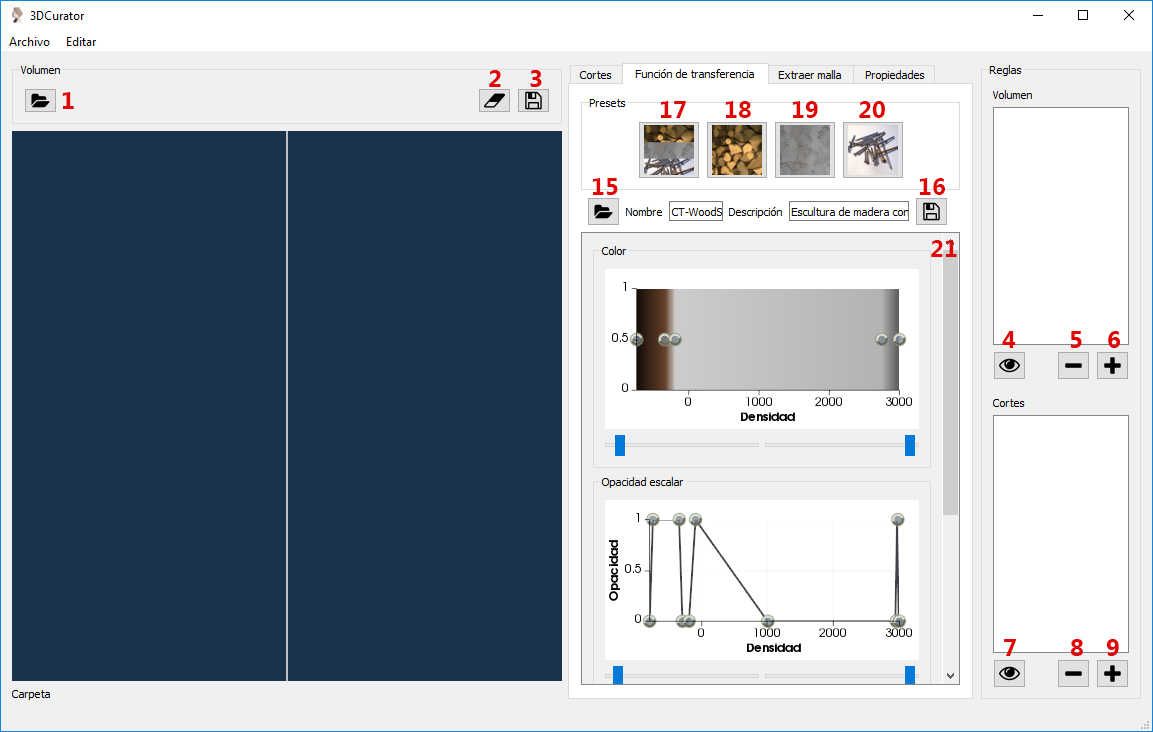
\includegraphics[width=12.5cm]{imagenes/gui_2}
	\caption{Captura de la GUI (Pestaña \textit{Función de transferencia})}
	\label{fig:gui_2}
\end{figure}

\begin{figure}[H]
	\centering
	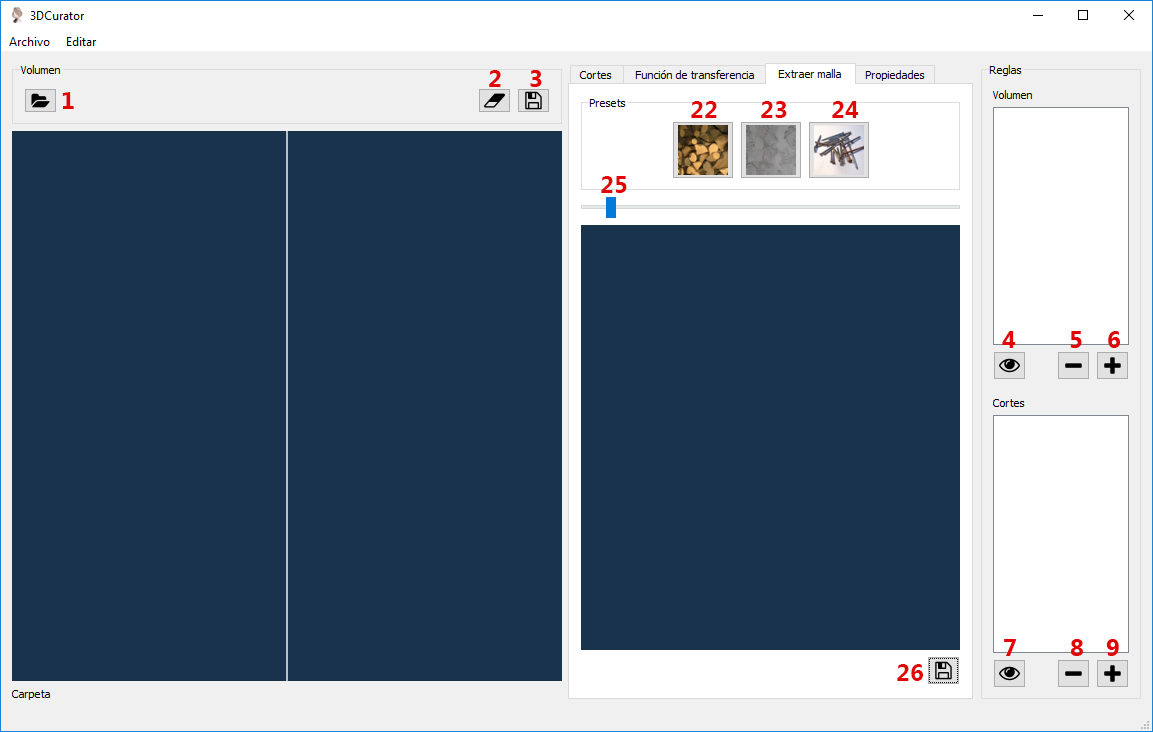
\includegraphics[width=12.5cm]{imagenes/gui_3}
	\caption{Captura de la GUI (Pestaña \textit{Extraer malla})}
	\label{fig:gui_3}
\end{figure}

\begin{figure}[H]
	\centering
	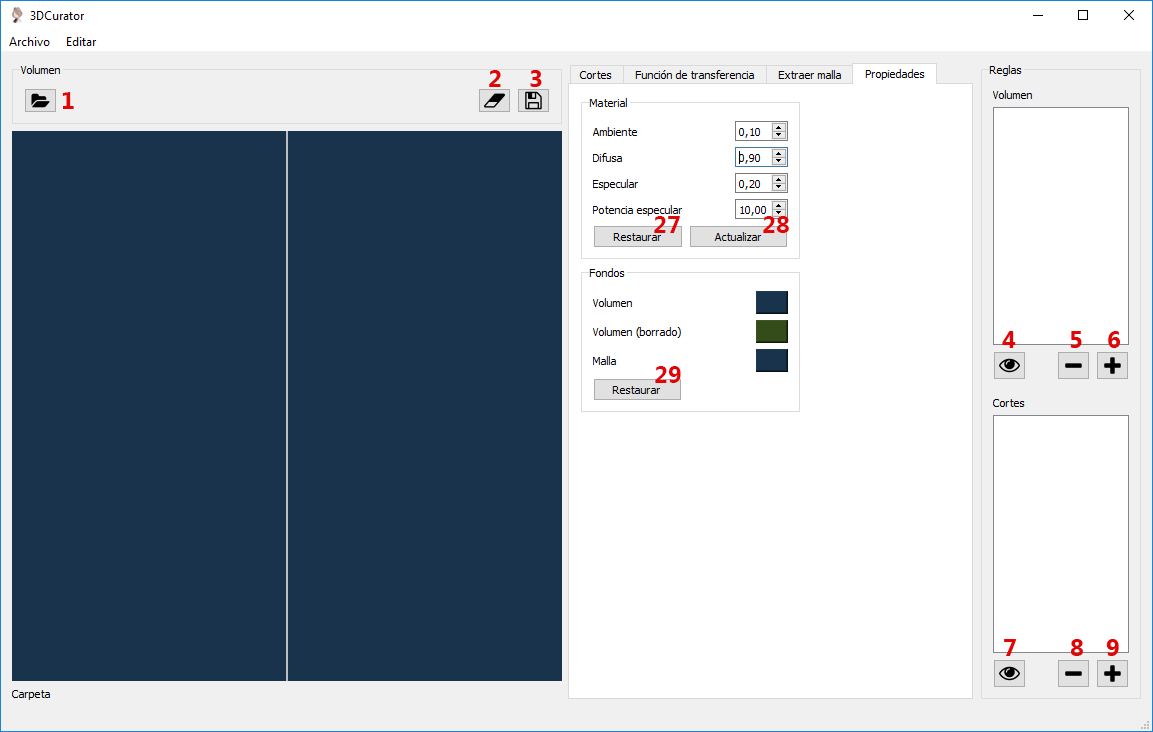
\includegraphics[width=12.5cm]{imagenes/gui_4}
	\caption{Captura de la GUI (Pestaña \textit{Propiedades})}
	\label{fig:gui_4}
\end{figure}

\section{Instrucciones de uso}

\subsection{Abrir directorio DICOM y visualizar datos}

Botón 1, Archivo $ \rangle $ Abrir... o \texttt{Ctrl+O}. Aparecerá una ventana donde se podrá elegir un directorio del sistema. Seleccionar aquel que tenga los archivos DICOM que se quieran importar y pulsar en abrir. Entonces empezará a cargar datos (puede tardar unos segundos). Si hay algún archivo en el directorio que no sea DICOM se mostrará un mensaje de error, pero si ha conseguido cargar el resto se puede continuar con la ejecución del programa sin problema.

Al abrir el archivo DICOM se mostrará la reconstrucción volumétrica en el visor principal, el corte producido con el plano en el visor del plano y la malla en el visor de la malla.

Si se mueve el ratón por el visor del corte abajo de este aparecerá el valor de densidad del pixel sobre el que está el ratón.

\subsubsection{Visor de volumen y malla}

\begin{itemize}
	\item \textbf{Girar cámara}: Click izdo. + arrastrar
	\item \textbf{Mover cámara}: Click central + arrastrar
	\item \textbf{Zoom}: Click dcho. + arrastrar o rueda del ratón
\end{itemize}

\subsubsection{Visor del corte}

\begin{itemize}
	\item \textbf{Mover}: Click central + arrastrar
	\item \textbf{Zoom}: Click dcho. + arrastrar o rueda del ratón
\end{itemize}

\subsection{Eliminar partes de la figura}

Botón 2, Editar $ \rangle $ Borrar partes o \texttt{Ctrl+May+D}. Se cambiará el visor del volumen de color y no se podrá girar la cámara.

Para borrar hacer click en un punto de la isla que se desea borrar. Entendiendo como isla parte que está separada de las demás. El proceso tardará unos segundos dependiendo del tamaño de la parte que se va a borrar. Al borrar se podrá ver el efecto del borrado y confirmar o volver a como estaba antes de borrar.

En ocasiones se necesitará hacer más de un borrado para borrar una isla por completo.

\subsection{Cambiar plano}

\subsubsection{Mostrar/Esconder}

En la pestaña \textit{Cortes} Botón 10, Editar $ \rangle $ Mostrar/Esconder plano o \texttt{Ctrl+May+H}. Esconderá o mostrará el plano en el visor de volumen. No se actualizará la imagen del corte si se ha escondido hasta que no se vuelva a mostrar.

\subsubsection{Posiciones por defecto}

Para colocarlas centradas en un plano anatómico:

\begin{itemize}
	\item \textbf{Sagital}: En la pestaña \textit{Cortes} Botón 11, Editar $ \rangle $ Plano sagital o \texttt{Ctrl+May+S}
	\item \textbf{Axial}: En la pestaña \textit{Cortes} Botón 12, Editar $ \rangle $ Plano axial o \texttt{Ctrl+May+A}
	\item \textbf{Coronal}: En la pestaña \textit{Cortes} Botón 13, Editar $ \rangle $ Plano coronal o \texttt{Ctrl+May+C}
\end{itemize}

\subsubsection{Mover}

El plano se mueve haciendo click derecho sobre éste y arrastrando hacia donde se desea. Para girarlo hacer el click en los extremos del plano.

\subsection{Guardar imagen del volumen}

Botón 3, Archivo $ \rangle $ Exportar figura... o \texttt{Ctrl+F}. Aparecerá una ventana donde se elegirá dónde, con qué nombre y con qué formato guardar la imagen.

\subsection{Guardar imagen del corte}

En la pestaña \textit{Cortes} Botón 14, Archivo $ \rangle $ Exportar corte... o \texttt{Ctrl+F}. Aparecerá una ventana donde se elegirá dónde, con qué nombre y con qué formato guardar la imagen.
 
\subsection{Cambiar color de fondo de visores}

En la pestaña \textit{Propiedades} pulsar sobre el botón coloreado a la derecha del nombre del visor cuyo color de fondo quiera ser cambiado. Aparecerá una ventana para elegir el color.

Si se desean restaurar los colores por defecto, pulsar en el Botón 29.

\subsection{Cambiar material del volumen}

En la pestaña \textit{Propiedades} cambiar los valores de las distintas componentes del material y pulsar en el Botón 28.

Si se desea restaurar el material por defecto, pulsar en el Botón 27.

\subsection{Función de transferencia}

\subsubsection{Cambiar \textit{preset}}

\begin{itemize}
	\item \textbf{Completo}: En la pestaña \textit{Función de transferencia} Botón 11, Editar $ \rangle $ Preset completo o \texttt{F1}
	\item \textbf{Madera}: En la pestaña \textit{Función de transferencia} Botón 12, Editar $ \rangle $ Preset madera o \texttt{F2}
	\item \textbf{Estuco}: En la pestaña \textit{Función de transferencia} Botón 13, Editar $ \rangle $ Preset estuco o \texttt{F3}
	\item \textbf{Metal}: En la pestaña \textit{Función de transferencia} Botón 14, Editar $ \rangle $ Preset metal o \texttt{F4}
\end{itemize}

\subsubsection{Importar}

En la pestaña \textit{Función de transferencia} Botón 15, Herramientas $ \rangle $ Importar preset... o \texttt{Ctrl+May+I}. Aparecerá una ventana donde se podrá escoger el archivo XML con el \textit{preset} que se quiere importar.

En la pestaña \textit{Propiedades} cambiar los valores de las distintas componentes del material y pulsar en el Botón 28.

Si se desea restaurar el material por defecto, pulsar en el Botón 27.

\subsubsection{Exportar}

Editar nombre y descripción en los campos dedicados para ello y, en la pestaña \textit{Función de transferencia} Botón 16, Herramientas $ \rangle $ Exportar preset... o \texttt{Ctrl+May+E}. Aparecerá una ventana donde se podrá escoger el nombre y la ubicación del archivo con el \textit{preset} que se exportará usando la función de transferencia actual.

\subsubsection{Editar}
 
Interactuar con las tres gráficas de la Caja 21 en la pestaña \textit{Función de transferencia}. Se puede cambiar el rango máximo y mínimo que aparece en la gráfica con los \textit{slider} inferiores. Para cambiar los puntos: 

\begin{itemize}
	\item \textbf{Añadir punto}: Click
	\item \textbf{Seleccionar punto}: Click sobre el punto
	\item \textbf{Eliminar punto}: Click central sobre el punto o seleccionar y \texttt{Del} o \texttt{Supr}.
	\item \textbf{Mover punto}: Seleccionar punto y arrastrar
	\item \textbf{Cambiar color}: (Solo en la de color) Doble click. Aparecerá una ventana de selección de color
\end{itemize}

\subsection{Generar malla}

En la pestaña \textit{Extraer malla} usar el Slider 25 para cambiar el valor de isosuperficie. Se generará en unos segundos la malla.

Para elegir entre cualquiera de los \textit{presets}:

\begin{itemize}
	\item \textbf{Madera}: En la pestaña \textit{Extraer malla} Botón 22, Editar $ \rangle $ Malla madera. Incluye los materiales madera, estuco y metal.
	\item \textbf{Estuco}: En la pestaña \textit{Extraer malla} Botón 23, Editar $ \rangle $ Malla estuco. Incluye los materiales estuco y metal.
	\item \textbf{Metal}: En la pestaña \textit{Extraer malla} Botón 24, Editar $ \rangle $ Malla metal. Incluye el material metal.
\end{itemize}

\subsection{Extraer malla}

En la pestaña \textit{Extraer malla} Botón 26, Herramientas $ \rangle $ Extraer malla... o \texttt{Ctrl+May+M}. Aparecerá una ventana donde se elegirá el nombre y la ubicación de la malla que se exportará en formato STL.

\subsection{Realizar medidas}

\subsubsection{Añadir regla}

Según el visor donde se realizará la medida pulsar el botón 6 (visor de volumen) o 9 (visor de cortes). Se hará click derecho en el punto inicial y en el final y aparecerá la medida en milímetros.

\subsubsection{Eliminar regla}

Seleccionar una regla de cualquiera de las cajas de reglas y pulsar en el botón 5 (reglas de volumen) u 8 (reglas de cortes). La regla desaparecerá.

\subsubsection{Mostrar/Esconder regla}

Seleccionar una regla de cualquiera de las cajas de reglas y pulsar en el botón 4 (reglas de volumen) u 7 (reglas de cortes). La regla se mostrará o se esconderá según su estado previo.

\subsubsection{Mover regla}

Click izquierdo en cualquiera de los puntos inicial o final de una regla y arrastrar el ratón.
%%\input{apendices/paper/paper}
%\input{glosario/entradas_glosario}
% \addcontentsline{toc}{chapter}{Glosario}
% \printglossary
%\chapter*{}
%\thispagestyle{empty}

\end{document}
